\documentclass[1p]{elsarticle_modified}
%\bibliographystyle{elsarticle-num}

%\usepackage[colorlinks]{hyperref}
%\usepackage{abbrmath_seonhwa} %\Abb, \Ascr, \Acal ,\Abf, \Afrak
\usepackage{amsfonts}
\usepackage{amssymb}
\usepackage{amsmath}
\usepackage{amsthm}
\usepackage{scalefnt}
\usepackage{amsbsy}
\usepackage{kotex}
\usepackage{caption}
\usepackage{subfig}
\usepackage{color}
\usepackage{graphicx}
\usepackage{xcolor} %% white, black, red, green, blue, cyan, magenta, yellow
\usepackage{float}
\usepackage{setspace}
\usepackage{hyperref}

\usepackage{tikz}
\usetikzlibrary{arrows}

\usepackage{multirow}
\usepackage{array} % fixed length table
\usepackage{hhline}

%%%%%%%%%%%%%%%%%%%%%
\makeatletter
\renewcommand*\env@matrix[1][\arraystretch]{%
	\edef\arraystretch{#1}%
	\hskip -\arraycolsep
	\let\@ifnextchar\new@ifnextchar
	\array{*\c@MaxMatrixCols c}}
\makeatother %https://tex.stackexchange.com/questions/14071/how-can-i-increase-the-line-spacing-in-a-matrix
%%%%%%%%%%%%%%%

\usepackage[normalem]{ulem}

\newcommand{\msout}[1]{\ifmmode\text{\sout{\ensuremath{#1}}}\else\sout{#1}\fi}
%SOURCE: \msout is \stkout macro in https://tex.stackexchange.com/questions/20609/strikeout-in-math-mode

\newcommand{\cancel}[1]{
	\ifmmode
	{\color{red}\msout{#1}}
	\else
	{\color{red}\sout{#1}}
	\fi
}

\newcommand{\add}[1]{
	{\color{blue}\uwave{#1}}
}

\newcommand{\replace}[2]{
	\ifmmode
	{\color{red}\msout{#1}}{\color{blue}\uwave{#2}}
	\else
	{\color{red}\sout{#1}}{\color{blue}\uwave{#2}}
	\fi
}

\newcommand{\Sol}{\mathcal{S}} %segment
\newcommand{\D}{D} %diagram
\newcommand{\A}{\mathcal{A}} %arc


%%%%%%%%%%%%%%%%%%%%%%%%%%%%%5 test

\def\sl{\operatorname{\textup{SL}}(2,\Cbb)}
\def\psl{\operatorname{\textup{PSL}}(2,\Cbb)}
\def\quan{\mkern 1mu \triangleright \mkern 1mu}

\theoremstyle{definition}
\newtheorem{thm}{Theorem}[section]
\newtheorem{prop}[thm]{Proposition}
\newtheorem{lem}[thm]{Lemma}
\newtheorem{ques}[thm]{Question}
\newtheorem{cor}[thm]{Corollary}
\newtheorem{defn}[thm]{Definition}
\newtheorem{exam}[thm]{Example}
\newtheorem{rmk}[thm]{Remark}
\newtheorem{alg}[thm]{Algorithm}

\newcommand{\I}{\sqrt{-1}}
\begin{document}

%\begin{frontmatter}
%
%\title{Boundary parabolic representations of knots up to 8 crossings}
%
%%% Group authors per affiliation:
%\author{Yunhi Cho} 
%\address{Department of Mathematics, University of Seoul, Seoul, Korea}
%\ead{yhcho@uos.ac.kr}
%
%
%\author{Seonhwa Kim} %\fnref{s_kim}}
%\address{Center for Geometry and Physics, Institute for Basic Science, Pohang, 37673, Korea}
%\ead{ryeona17@ibs.re.kr}
%
%\author{Hyuk Kim}
%\address{Department of Mathematical Sciences, Seoul National University, Seoul 08826, Korea}
%\ead{hyukkim@snu.ac.kr}
%
%\author{Seokbeom Yoon}
%\address{Department of Mathematical Sciences, Seoul National University, Seoul, 08826,  Korea}
%\ead{sbyoon15@snu.ac.kr}
%
%\begin{abstract}
%We find all boundary parabolic representation of knots up to 8 crossings.
%
%\end{abstract}
%\begin{keyword}
%    \MSC[2010] 57M25 
%\end{keyword}
%
%\end{frontmatter}

%\linenumbers
%\tableofcontents
%
\newcommand\colored[1]{\textcolor{white}{\rule[-0.35ex]{0.8em}{1.4ex}}\kern-0.8em\color{red} #1}%
%\newcommand\colored[1]{\textcolor{white}{ #1}\kern-2.17ex	\textcolor{white}{ #1}\kern-1.81ex	\textcolor{white}{ #1}\kern-2.15ex\color{red}#1	}

{\Large $\underline{11n_{165}~(K11n_{165})}$}

\setlength{\tabcolsep}{10pt}
\renewcommand{\arraystretch}{1.6}
\vspace{1cm}\begin{tabular}{m{100pt}>{\centering\arraybackslash}m{274pt}}
\multirow{5}{120pt}{
	\centering
	\includegraphics[width=112pt]{../../../GIT/diagram.site/Diagrams/png/781_11n_165.png}\\
\ \ \ A knot diagram\footnotemark}&
\allowdisplaybreaks
\textbf{Linearized knot diagam} \\
\cline{2-2}
 &
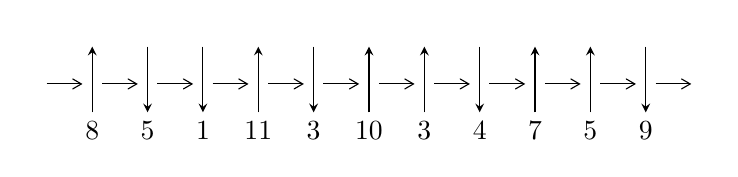
\begin{tikzpicture}[x=20pt, y=17pt]
	% nodes
	\node (C0) at (0, 0) {};
	\node (C1) at (1, 0) {};
	\node (C1U) at (1, +1) {};
	\node (C1D) at (1, -1) {8};

	\node (C2) at (2, 0) {};
	\node (C2U) at (2, +1) {};
	\node (C2D) at (2, -1) {5};

	\node (C3) at (3, 0) {};
	\node (C3U) at (3, +1) {};
	\node (C3D) at (3, -1) {1};

	\node (C4) at (4, 0) {};
	\node (C4U) at (4, +1) {};
	\node (C4D) at (4, -1) {11};

	\node (C5) at (5, 0) {};
	\node (C5U) at (5, +1) {};
	\node (C5D) at (5, -1) {3};

	\node (C6) at (6, 0) {};
	\node (C6U) at (6, +1) {};
	\node (C6D) at (6, -1) {10};

	\node (C7) at (7, 0) {};
	\node (C7U) at (7, +1) {};
	\node (C7D) at (7, -1) {3};

	\node (C8) at (8, 0) {};
	\node (C8U) at (8, +1) {};
	\node (C8D) at (8, -1) {4};

	\node (C9) at (9, 0) {};
	\node (C9U) at (9, +1) {};
	\node (C9D) at (9, -1) {7};

	\node (C10) at (10, 0) {};
	\node (C10U) at (10, +1) {};
	\node (C10D) at (10, -1) {5};

	\node (C11) at (11, 0) {};
	\node (C11U) at (11, +1) {};
	\node (C11D) at (11, -1) {9};
	\node (C12) at (12, 0) {};

	% arrows
	\draw[->,>={angle 60}]
	(C0) edge (C1) (C1) edge (C2) (C2) edge (C3) (C3) edge (C4) (C4) edge (C5) (C5) edge (C6) (C6) edge (C7) (C7) edge (C8) (C8) edge (C9) (C9) edge (C10) (C10) edge (C11) (C11) edge (C12) ;	\draw[->,>=stealth]
	(C1D) edge (C1U) (C2U) edge (C2D) (C3U) edge (C3D) (C4D) edge (C4U) (C5U) edge (C5D) (C6D) edge (C6U) (C7D) edge (C7U) (C8U) edge (C8D) (C9D) edge (C9U) (C10D) edge (C10U) (C11U) edge (C11D) ;
	\end{tikzpicture} \\
\hhline{~~} \\& 
\textbf{Solving Sequence} \\ \cline{2-2} 
 &
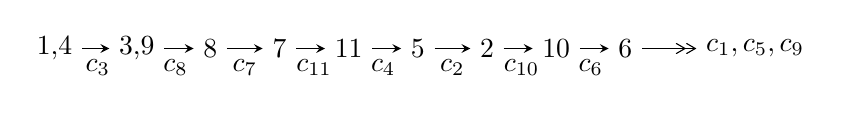
\begin{tikzpicture}[x=25pt, y=7pt]
	% node
	\node (A0) at (-1/8, 0) {1,4};
	\node (A1) at (17/16, 0) {3,9};
	\node (A2) at (17/8, 0) {8};
	\node (A3) at (25/8, 0) {7};
	\node (A4) at (33/8, 0) {11};
	\node (A5) at (41/8, 0) {5};
	\node (A6) at (49/8, 0) {2};
	\node (A7) at (57/8, 0) {10};
	\node (A8) at (65/8, 0) {6};
	\node (C1) at (1/2, -1) {$c_{3}$};
	\node (C2) at (13/8, -1) {$c_{8}$};
	\node (C3) at (21/8, -1) {$c_{7}$};
	\node (C4) at (29/8, -1) {$c_{11}$};
	\node (C5) at (37/8, -1) {$c_{4}$};
	\node (C6) at (45/8, -1) {$c_{2}$};
	\node (C7) at (53/8, -1) {$c_{10}$};
	\node (C8) at (61/8, -1) {$c_{6}$};
	\node (A9) at (10, 0) {$c_{1},c_{5},c_{9}$};

	% edge
	\draw[->,>=stealth]	
	(A0) edge (A1) (A1) edge (A2) (A2) edge (A3) (A3) edge (A4) (A4) edge (A5) (A5) edge (A6) (A6) edge (A7) (A7) edge (A8) ;
	\draw[->>,>={angle 60}]	
	(A8) edge (A9);
\end{tikzpicture} \\ 

\end{tabular} \\

\footnotetext{
The image of knot diagram is generated by the software ``\textbf{Draw programme}" developed by Andrew Bartholomew(\url{http://www.layer8.co.uk/maths/draw/index.htm\#Running-draw}), where we modified some parts for our purpose(\url{https://github.com/CATsTAILs/LinksPainter}).
}\phantom \\ \newline 
\centering \textbf{Ideals for irreducible components\footnotemark of $X_{\text{par}}$} 
 
\begin{align*}
I^u_{1}&=\langle 
-766790 u^{19}+10314727 u^{18}+\cdots+1340393 b-9262246,\\
\phantom{I^u_{1}}&\phantom{= \langle  }-9262246 u^{19}+139639714 u^{18}+\cdots+17425109 a+534767514,\;u^{20}-14 u^{19}+\cdots-140 u+13\rangle \\
I^u_{2}&=\langle 
- a^3 u^3+4 u^3 a^2+\cdots+75 a-12,\\
\phantom{I^u_{2}}&\phantom{= \langle  }- a^3 u^2+a^4-2 a^3 u+3 a^2 u^2-2 u^3 a-2 a^3+5 a^2 u-4 u^2 a+u^3+5 a^2-5 a u- u^2- a-3 u-6,\\
\phantom{I^u_{2}}&\phantom{= \langle  }u^4+u^3+u^2- u+1\rangle \\
I^u_{3}&=\langle 
25 u^{11}+234 u^{10}+\cdots+167 b+63,\;-63 u^{11}-416 u^{10}+\cdots+167 a+55,\\
\phantom{I^u_{3}}&\phantom{= \langle  }u^{12}+7 u^{11}+26 u^{10}+60 u^9+91 u^8+87 u^7+46 u^6+5 u^5-5 u^4- u^3+u^2+1\rangle \\
I^u_{4}&=\langle 
u^3- a u+u^2+b-1,\;- u^3 a-3 u^2 a- u^3+a^2-3 a u-3 u^2- a-4 u-2,\;u^4+2 u^3+2 u^2+u+1\rangle \\
I^u_{5}&=\langle 
- u^3- a u-2 u^2+b-2 u,\;u^2 a+a^2+2 a u+2 a-1,\;u^4+2 u^3+2 u^2+u+1\rangle \\
\\
I^v_{1}&=\langle 
a,\;b^2+b+1,\;v-1\rangle \\
\end{align*}
\raggedright * 6 irreducible components of $\dim_{\mathbb{C}}=0$, with total 66 representations.\\
\footnotetext{All coefficients of polynomials are rational numbers. But the coefficients are sometimes approximated in decimal forms when there is not enough margin.}
\newpage
\renewcommand{\arraystretch}{1}
\centering \section*{I. $I^u_{1}= \langle -7.67\times10^{5} u^{19}+1.03\times10^{7} u^{18}+\cdots+1.34\times10^{6} b-9.26\times10^{6},\;-9.26\times10^{6} u^{19}+1.40\times10^{8} u^{18}+\cdots+1.74\times10^{7} a+5.35\times10^{8},\;u^{20}-14 u^{19}+\cdots-140 u+13 \rangle$}
\flushleft \textbf{(i) Arc colorings}\\
\begin{tabular}{m{7pt} m{180pt} m{7pt} m{180pt} }
\flushright $a_{1}=$&$\begin{pmatrix}0\\u\end{pmatrix}$ \\
\flushright $a_{4}=$&$\begin{pmatrix}1\\0\end{pmatrix}$ \\
\flushright $a_{3}=$&$\begin{pmatrix}1\\- u^2\end{pmatrix}$ \\
\flushright $a_{9}=$&$\begin{pmatrix}0.531546 u^{19}-8.01371 u^{18}+\cdots+299.293 u-30.6895\\0.572064 u^{19}-7.69530 u^{18}+\cdots-43.7270 u+6.91010\end{pmatrix}$ \\
\flushright $a_{8}=$&$\begin{pmatrix}1.10361 u^{19}-15.7090 u^{18}+\cdots+255.567 u-23.7794\\0.572064 u^{19}-7.69530 u^{18}+\cdots-43.7270 u+6.91010\end{pmatrix}$ \\
\flushright $a_{7}=$&$\begin{pmatrix}1.60433 u^{19}-22.5319 u^{18}+\cdots+349.827 u-34.0496\\1.31746 u^{19}-15.8315 u^{18}+\cdots-63.4249 u+9.34363\end{pmatrix}$ \\
\flushright $a_{11}=$&$\begin{pmatrix}1.03159 u^{19}-13.4015 u^{18}+\cdots+183.124 u-20.5381\\-1.04074 u^{19}+13.5128 u^{18}+\cdots-122.884 u+13.4107\end{pmatrix}$ \\
\flushright $a_{5}=$&$\begin{pmatrix}1.71042 u^{19}-22.8588 u^{18}+\cdots+203.782 u-20.2563\\-0.0294787 u^{19}+1.23697 u^{18}+\cdots-85.9094 u+8.70582\end{pmatrix}$ \\
\flushright $a_{2}=$&$\begin{pmatrix}0.00767507 u^{19}-0.391944 u^{18}+\cdots+67.6479 u-7.24644\\0.0168279 u^{19}-0.503255 u^{18}+\cdots+9.40885 u-0.118987\end{pmatrix}$ \\
\flushright $a_{10}=$&$\begin{pmatrix}-0.0194671 u^{19}-1.23452 u^{18}+\cdots+309.121 u-35.2533\\1.74036 u^{19}-23.1238 u^{18}+\cdots+166.693 u-14.1659\end{pmatrix}$ \\
\flushright $a_{6}=$&$\begin{pmatrix}-1.77426 u^{19}+23.5639 u^{18}+\cdots-159.740 u+14.8304\\-0.0610127 u^{19}-0.487643 u^{18}+\cdots+111.512 u-11.1602\end{pmatrix}$\\ \flushright $a_{6}=$&$\begin{pmatrix}-1.77426 u^{19}+23.5639 u^{18}+\cdots-159.740 u+14.8304\\-0.0610127 u^{19}-0.487643 u^{18}+\cdots+111.512 u-11.1602\end{pmatrix}$\\&\end{tabular}
\flushleft \textbf{(ii) Obstruction class $= -1$}\\~\\
\flushleft \textbf{(iii) Cusp Shapes $= -\frac{2833789}{1340393} u^{19}+\frac{38974772}{1340393} u^{18}+\cdots-\frac{300276118}{1340393} u+\frac{19362744}{1340393}$}\\~\\
\newpage\renewcommand{\arraystretch}{1}
\flushleft \textbf{(iv) u-Polynomials at the component}\newline \\
\begin{tabular}{m{50pt}|m{274pt}}
Crossings & \hspace{64pt}u-Polynomials at each crossing \\
\hline $$\begin{aligned}c_{1}\end{aligned}$$&$\begin{aligned}
&u^{20}- u^{19}+\cdots-4 u+1
\end{aligned}$\\
\hline $$\begin{aligned}c_{2},c_{5}\end{aligned}$$&$\begin{aligned}
&u^{20}+u^{19}+\cdots+2 u+1
\end{aligned}$\\
\hline $$\begin{aligned}c_{3}\end{aligned}$$&$\begin{aligned}
&u^{20}-14 u^{19}+\cdots-140 u+13
\end{aligned}$\\
\hline $$\begin{aligned}c_{4},c_{10}\end{aligned}$$&$\begin{aligned}
&u^{20}-14 u^{19}+\cdots-2560 u+256
\end{aligned}$\\
\hline $$\begin{aligned}c_{6},c_{9}\end{aligned}$$&$\begin{aligned}
&u^{20}+9 u^{19}+\cdots+28 u+13
\end{aligned}$\\
\hline $$\begin{aligned}c_{7}\end{aligned}$$&$\begin{aligned}
&u^{20}+u^{19}+\cdots+17 u+21
\end{aligned}$\\
\hline $$\begin{aligned}c_{8},c_{11}\end{aligned}$$&$\begin{aligned}
&u^{20}-2 u^{19}+\cdots-4 u+1
\end{aligned}$\\
\hline
\end{tabular}\\~\\
\newpage\renewcommand{\arraystretch}{1}
\flushleft \textbf{(v) Riley Polynomials at the component}\newline \\
\begin{tabular}{m{50pt}|m{274pt}}
Crossings & \hspace{64pt}Riley Polynomials at each crossing \\
\hline $$\begin{aligned}c_{1}\end{aligned}$$&$\begin{aligned}
&y^{20}-5 y^{19}+\cdots-14 y+1
\end{aligned}$\\
\hline $$\begin{aligned}c_{2},c_{5}\end{aligned}$$&$\begin{aligned}
&y^{20}+23 y^{19}+\cdots+10 y+1
\end{aligned}$\\
\hline $$\begin{aligned}c_{3}\end{aligned}$$&$\begin{aligned}
&y^{20}+4 y^{19}+\cdots+498 y+169
\end{aligned}$\\
\hline $$\begin{aligned}c_{4},c_{10}\end{aligned}$$&$\begin{aligned}
&y^{20}+12 y^{19}+\cdots-65536 y+65536
\end{aligned}$\\
\hline $$\begin{aligned}c_{6},c_{9}\end{aligned}$$&$\begin{aligned}
&y^{20}+9 y^{19}+\cdots+698 y+169
\end{aligned}$\\
\hline $$\begin{aligned}c_{7}\end{aligned}$$&$\begin{aligned}
&y^{20}-19 y^{19}+\cdots-2641 y+441
\end{aligned}$\\
\hline $$\begin{aligned}c_{8},c_{11}\end{aligned}$$&$\begin{aligned}
&y^{20}+20 y^{18}+\cdots+4 y+1
\end{aligned}$\\
\hline
\end{tabular}\\~\\
\newpage\flushleft \textbf{(vi) Complex Volumes and Cusp Shapes}
$$\begin{array}{c|c|c}  
\text{Solutions to }I^u_{1}& \I (\text{vol} + \sqrt{-1}CS) & \text{Cusp shape}\\
 \hline 
\begin{aligned}
u &= \phantom{-}0.643832 + 0.539702 I \\
a &= -1.74604 + 0.04327 I \\
b &= \phantom{-}1.14751 + 0.91448 I\end{aligned}
 & -7.56901 - 4.35325 I & \phantom{-}6.00959 - 2.36650 I \\ \hline\begin{aligned}
u &= \phantom{-}0.643832 - 0.539702 I \\
a &= -1.74604 - 0.04327 I \\
b &= \phantom{-}1.14751 - 0.91448 I\end{aligned}
 & -7.56901 + 4.35325 I & \phantom{-}6.00959 + 2.36650 I \\ \hline\begin{aligned}
u &= \phantom{-}1.198930 + 0.321628 I \\
a &= \phantom{-}0.470312 - 0.608504 I \\
b &= -0.759582 + 0.578288 I\end{aligned}
 & \phantom{-}0.87661 + 1.80368 I & -0.33009 - 3.39562 I \\ \hline\begin{aligned}
u &= \phantom{-}1.198930 - 0.321628 I \\
a &= \phantom{-}0.470312 + 0.608504 I \\
b &= -0.759582 - 0.578288 I\end{aligned}
 & \phantom{-}0.87661 - 1.80368 I & -0.33009 + 3.39562 I \\ \hline\begin{aligned}
u &= \phantom{-}0.808778 + 1.074790 I \\
a &= \phantom{-}1.154450 - 0.190358 I \\
b &= -1.13829 - 1.08683 I\end{aligned}
 & \phantom{-}2.70163 - 8.25419 I & \phantom{-}1.74639 + 5.26030 I \\ \hline\begin{aligned}
u &= \phantom{-}0.808778 - 1.074790 I \\
a &= \phantom{-}1.154450 + 0.190358 I \\
b &= -1.13829 + 1.08683 I\end{aligned}
 & \phantom{-}2.70163 + 8.25419 I & \phantom{-}1.74639 - 5.26030 I \\ \hline\begin{aligned}
u &= -0.081606 + 0.559081 I \\
a &= -1.233730 + 0.525348 I \\
b &= \phantom{-}0.193032 + 0.732624 I\end{aligned}
 & \phantom{-}1.06285 + 1.12930 I & \phantom{-}5.13966 - 4.07834 I \\ \hline\begin{aligned}
u &= -0.081606 - 0.559081 I \\
a &= -1.233730 - 0.525348 I \\
b &= \phantom{-}0.193032 - 0.732624 I\end{aligned}
 & \phantom{-}1.06285 - 1.12930 I & \phantom{-}5.13966 + 4.07834 I \\ \hline\begin{aligned}
u &= \phantom{-}0.80616 + 1.24885 I \\
a &= -0.724968 - 0.008424 I \\
b &= \phantom{-}0.573922 + 0.912168 I\end{aligned}
 & \phantom{-}6.49001 - 1.26443 I & \phantom{-}4.97798 + 1.96291 I \\ \hline\begin{aligned}
u &= \phantom{-}0.80616 - 1.24885 I \\
a &= -0.724968 + 0.008424 I \\
b &= \phantom{-}0.573922 - 0.912168 I\end{aligned}
 & \phantom{-}6.49001 + 1.26443 I & \phantom{-}4.97798 - 1.96291 I\\
 \hline 
 \end{array}$$\newpage$$\begin{array}{c|c|c}  
\text{Solutions to }I^u_{1}& \I (\text{vol} + \sqrt{-1}CS) & \text{Cusp shape}\\
 \hline 
\begin{aligned}
u &= \phantom{-}1.01334 + 1.17077 I \\
a &= -1.029040 + 0.119371 I \\
b &= \phantom{-}1.18252 + 1.08380 I\end{aligned}
 & \phantom{-}1.5683 - 15.8169 I & -0.23034 + 8.70601 I \\ \hline\begin{aligned}
u &= \phantom{-}1.01334 - 1.17077 I \\
a &= -1.029040 - 0.119371 I \\
b &= \phantom{-}1.18252 - 1.08380 I\end{aligned}
 & \phantom{-}1.5683 + 15.8169 I & -0.23034 - 8.70601 I \\ \hline\begin{aligned}
u &= \phantom{-}0.307600 + 0.248640 I \\
a &= \phantom{-}2.41339 + 0.42231 I \\
b &= -0.637356 - 0.729970 I\end{aligned}
 & -0.01507 - 1.86524 I & \phantom{-}0.60762 + 4.36679 I \\ \hline\begin{aligned}
u &= \phantom{-}0.307600 - 0.248640 I \\
a &= \phantom{-}2.41339 - 0.42231 I \\
b &= -0.637356 + 0.729970 I\end{aligned}
 & -0.01507 + 1.86524 I & \phantom{-}0.60762 - 4.36679 I \\ \hline\begin{aligned}
u &= -0.34327 + 1.61845 I \\
a &= \phantom{-}0.214787 + 0.114493 I \\
b &= \phantom{-}0.259032 - 0.308320 I\end{aligned}
 & -4.19435 + 1.15765 I & \phantom{-}2.14031 - 7.95914 I \\ \hline\begin{aligned}
u &= -0.34327 - 1.61845 I \\
a &= \phantom{-}0.214787 - 0.114493 I \\
b &= \phantom{-}0.259032 + 0.308320 I\end{aligned}
 & -4.19435 - 1.15765 I & \phantom{-}2.14031 + 7.95914 I \\ \hline\begin{aligned}
u &= \phantom{-}1.15645 + 1.28057 I \\
a &= \phantom{-}0.604483 + 0.080235 I \\
b &= -0.596309 - 0.866871 I\end{aligned}
 & \phantom{-}5.15014 - 7.97058 I & \phantom{-}2.89077 + 7.60145 I \\ \hline\begin{aligned}
u &= \phantom{-}1.15645 - 1.28057 I \\
a &= \phantom{-}0.604483 - 0.080235 I \\
b &= -0.596309 + 0.866871 I\end{aligned}
 & \phantom{-}5.15014 + 7.97058 I & \phantom{-}2.89077 - 7.60145 I \\ \hline\begin{aligned}
u &= \phantom{-}1.48978 + 0.91920 I \\
a &= -0.277498 + 0.393931 I \\
b &= \phantom{-}0.775515 - 0.331794 I\end{aligned}
 & \phantom{-}0.50861 + 7.39141 I & -3.95189 - 9.17426 I \\ \hline\begin{aligned}
u &= \phantom{-}1.48978 - 0.91920 I \\
a &= -0.277498 - 0.393931 I \\
b &= \phantom{-}0.775515 + 0.331794 I\end{aligned}
 & \phantom{-}0.50861 - 7.39141 I & -3.95189 + 9.17426 I\\
 \hline 
 \end{array}$$\newpage\newpage\renewcommand{\arraystretch}{1}
\centering \section*{II. $I^u_{2}= \langle - a^3 u^3+4 u^3 a^2+\cdots+75 a-12,\;-2 u^3 a+u^3+\cdots- a-6,\;u^4+u^3+u^2- u+1 \rangle$}
\flushleft \textbf{(i) Arc colorings}\\
\begin{tabular}{m{7pt} m{180pt} m{7pt} m{180pt} }
\flushright $a_{1}=$&$\begin{pmatrix}0\\u\end{pmatrix}$ \\
\flushright $a_{4}=$&$\begin{pmatrix}1\\0\end{pmatrix}$ \\
\flushright $a_{3}=$&$\begin{pmatrix}1\\- u^2\end{pmatrix}$ \\
\flushright $a_{9}=$&$\begin{pmatrix}a\\\frac{1}{45} a^3 u^3-\frac{4}{45} u^3 a^2+\cdots-\frac{5}{3} a+\frac{4}{15}\end{pmatrix}$ \\
\flushright $a_{8}=$&$\begin{pmatrix}\frac{1}{45} a^3 u^3-\frac{4}{45} u^3 a^2+\cdots-\frac{2}{3} a+\frac{4}{15}\\\frac{1}{45} a^3 u^3-\frac{4}{45} u^3 a^2+\cdots-\frac{5}{3} a+\frac{4}{15}\end{pmatrix}$ \\
\flushright $a_{7}=$&$\begin{pmatrix}0.244444 a^{3} u^{3}+0.0222222 a^{2} u^{3}+\cdots+0.666667 a-0.0666667\\\frac{7}{15} a^3 u^3-\frac{13}{15} u^3 a^2+\cdots- a+\frac{3}{5}\end{pmatrix}$ \\
\flushright $a_{11}=$&$\begin{pmatrix}a^2 u\\-0.244444 a^{3} u^{3}-0.0222222 a^{2} u^{3}+\cdots+0.333333 a-0.933333\end{pmatrix}$ \\
\flushright $a_{5}=$&$\begin{pmatrix}\frac{2}{45} a^3 u^3-\frac{8}{45} u^3 a^2+\cdots-\frac{1}{3} a+\frac{8}{15}\\-0.244444 a^{3} u^{3}-0.0222222 a^{2} u^{3}+\cdots+0.333333 a+0.0666667\end{pmatrix}$ \\
\flushright $a_{2}=$&$\begin{pmatrix}-0.688889 a^{3} u^{3}-0.244444 a^{2} u^{3}+\cdots-0.333333 a-0.266667\\-\frac{4}{9} a^3 u^3-\frac{2}{9} u^3 a^2+\cdots-\frac{2}{3} a+\frac{2}{3}\end{pmatrix}$ \\
\flushright $a_{10}=$&$\begin{pmatrix}0.288889 a^{3} u^{3}-0.155556 a^{2} u^{3}+\cdots-0.666667 a+0.466667\\-0.244444 a^{3} u^{3}-0.0222222 a^{2} u^{3}+\cdots+0.333333 a+0.0666667\end{pmatrix}$ \\
\flushright $a_{6}=$&$\begin{pmatrix}\frac{2}{9} a^3 u^3+\frac{1}{9} u^3 a^2+\cdots+\frac{1}{3} a-\frac{1}{3}\\0.177778 a^{3} u^{3}-0.711111 a^{2} u^{3}+\cdots-0.333333 a+0.133333\end{pmatrix}$\\ \flushright $a_{6}=$&$\begin{pmatrix}\frac{2}{9} a^3 u^3+\frac{1}{9} u^3 a^2+\cdots+\frac{1}{3} a-\frac{1}{3}\\0.177778 a^{3} u^{3}-0.711111 a^{2} u^{3}+\cdots-0.333333 a+0.133333\end{pmatrix}$\\&\end{tabular}
\flushleft \textbf{(ii) Obstruction class $= -1$}\\~\\
\flushleft \textbf{(iii) Cusp Shapes $= -\frac{44}{45} a^3 u^3-\frac{76}{45} a^3 u^2-\frac{4}{45} u^3 a^2+\frac{16}{15} a^3 u+\frac{124}{45} a^2 u^2-\frac{4}{3} u^3 a-\frac{52}{45} a^3-\frac{4}{15} a^2 u-\frac{8}{3} u^2 a+\frac{68}{15} u^3+\frac{28}{45} a^2-4 a u+\frac{172}{15} u^2+\frac{4}{3} a+\frac{48}{5} u-\frac{26}{15}$}\\~\\
\newpage\renewcommand{\arraystretch}{1}
\flushleft \textbf{(iv) u-Polynomials at the component}\newline \\
\begin{tabular}{m{50pt}|m{274pt}}
Crossings & \hspace{64pt}u-Polynomials at each crossing \\
\hline $$\begin{aligned}c_{1}\end{aligned}$$&$\begin{aligned}
&u^{16}+2 u^{15}+\cdots+10 u+25
\end{aligned}$\\
\hline $$\begin{aligned}c_{2},c_{5}\end{aligned}$$&$\begin{aligned}
&u^{16}- u^{15}+\cdots-12 u+3
\end{aligned}$\\
\hline $$\begin{aligned}c_{3}\end{aligned}$$&$\begin{aligned}
&(u^4+u^3+u^2- u+1)^4
\end{aligned}$\\
\hline $$\begin{aligned}c_{4},c_{10}\end{aligned}$$&$\begin{aligned}
&(u^2+u+1)^8
\end{aligned}$\\
\hline $$\begin{aligned}c_{6},c_{9}\end{aligned}$$&$\begin{aligned}
&(u^4- u^3+u^2+u+1)^4
\end{aligned}$\\
\hline $$\begin{aligned}c_{7}\end{aligned}$$&$\begin{aligned}
&u^{16}-2 u^{15}+\cdots+264 u+111
\end{aligned}$\\
\hline $$\begin{aligned}c_{8},c_{11}\end{aligned}$$&$\begin{aligned}
&u^{16}+u^{15}+\cdots-12 u+3
\end{aligned}$\\
\hline
\end{tabular}\\~\\
\newpage\renewcommand{\arraystretch}{1}
\flushleft \textbf{(v) Riley Polynomials at the component}\newline \\
\begin{tabular}{m{50pt}|m{274pt}}
Crossings & \hspace{64pt}Riley Polynomials at each crossing \\
\hline $$\begin{aligned}c_{1}\end{aligned}$$&$\begin{aligned}
&y^{16}+34 y^{14}+\cdots-4150 y+625
\end{aligned}$\\
\hline $$\begin{aligned}c_{2},c_{5}\end{aligned}$$&$\begin{aligned}
&y^{16}+3 y^{15}+\cdots+402 y+9
\end{aligned}$\\
\hline $$\begin{aligned}c_{3},c_{6},c_{9}\end{aligned}$$&$\begin{aligned}
&(y^4+y^3+5 y^2+y+1)^4
\end{aligned}$\\
\hline $$\begin{aligned}c_{4},c_{10}\end{aligned}$$&$\begin{aligned}
&(y^2+y+1)^8
\end{aligned}$\\
\hline $$\begin{aligned}c_{7}\end{aligned}$$&$\begin{aligned}
&y^{16}-16 y^{15}+\cdots-83682 y+12321
\end{aligned}$\\
\hline $$\begin{aligned}c_{8},c_{11}\end{aligned}$$&$\begin{aligned}
&y^{16}-5 y^{15}+\cdots-102 y+9
\end{aligned}$\\
\hline
\end{tabular}\\~\\
\newpage\flushleft \textbf{(vi) Complex Volumes and Cusp Shapes}
$$\begin{array}{c|c|c}  
\text{Solutions to }I^u_{2}& \I (\text{vol} + \sqrt{-1}CS) & \text{Cusp shape}\\
 \hline 
\begin{aligned}
u &= \phantom{-}0.433380 + 0.525827 I \\
a &= -0.671245 + 0.201645 I \\
b &= \phantom{-}1.22825 - 1.67883 I\end{aligned}
 & \phantom{-}2.24108 - 6.71592 I & \phantom{-}1.29059 + 13.74348 I \\ \hline\begin{aligned}
u &= \phantom{-}0.433380 + 0.525827 I \\
a &= \phantom{-}1.48035 + 0.37541 I \\
b &= -1.59236 + 0.24028 I\end{aligned}
 & \phantom{-}2.24108 - 2.65615 I & \phantom{-}1.29059 + 6.81528 I \\ \hline\begin{aligned}
u &= \phantom{-}0.433380 + 0.525827 I \\
a &= \phantom{-}1.21416 - 2.02760 I \\
b &= -0.444152 - 0.941106 I\end{aligned}
 & \phantom{-}2.24108 - 2.65615 I & \phantom{-}1.29059 + 6.81528 I \\ \hline\begin{aligned}
u &= \phantom{-}0.433380 + 0.525827 I \\
a &= \phantom{-}0.75482 + 2.95796 I \\
b &= \phantom{-}0.396935 + 0.265570 I\end{aligned}
 & \phantom{-}2.24108 - 6.71592 I & \phantom{-}1.29059 + 13.74348 I \\ \hline\begin{aligned}
u &= \phantom{-}0.433380 - 0.525827 I \\
a &= -0.671245 - 0.201645 I \\
b &= \phantom{-}1.22825 + 1.67883 I\end{aligned}
 & \phantom{-}2.24108 + 6.71592 I & \phantom{-}1.29059 - 13.74348 I \\ \hline\begin{aligned}
u &= \phantom{-}0.433380 - 0.525827 I \\
a &= \phantom{-}1.48035 - 0.37541 I \\
b &= -1.59236 - 0.24028 I\end{aligned}
 & \phantom{-}2.24108 + 2.65615 I & \phantom{-}1.29059 - 6.81528 I \\ \hline\begin{aligned}
u &= \phantom{-}0.433380 - 0.525827 I \\
a &= \phantom{-}1.21416 + 2.02760 I \\
b &= -0.444152 + 0.941106 I\end{aligned}
 & \phantom{-}2.24108 + 2.65615 I & \phantom{-}1.29059 - 6.81528 I \\ \hline\begin{aligned}
u &= \phantom{-}0.433380 - 0.525827 I \\
a &= \phantom{-}0.75482 - 2.95796 I \\
b &= \phantom{-}0.396935 - 0.265570 I\end{aligned}
 & \phantom{-}2.24108 + 6.71592 I & \phantom{-}1.29059 - 13.74348 I \\ \hline\begin{aligned}
u &= -0.93338 + 1.13249 I \\
a &= \phantom{-}0.937489 + 0.356410 I \\
b &= -0.928296 + 1.033700 I\end{aligned}
 & -2.24108 + 6.71592 I & -1.29059 - 13.74348 I \\ \hline\begin{aligned}
u &= -0.93338 + 1.13249 I \\
a &= -0.945855 - 0.040136 I \\
b &= \phantom{-}1.27866 - 0.72903 I\end{aligned}
 & -2.24108 + 6.71592 I & -1.29059 - 13.74348 I\\
 \hline 
 \end{array}$$\newpage$$\begin{array}{c|c|c}  
\text{Solutions to }I^u_{2}& \I (\text{vol} + \sqrt{-1}CS) & \text{Cusp shape}\\
 \hline 
\begin{aligned}
u &= -0.93338 + 1.13249 I \\
a &= -0.556441 - 0.371428 I \\
b &= \phantom{-}0.500964 - 0.132390 I\end{aligned}
 & -2.24108 + 2.65615 I & -1.29059 - 6.81528 I \\ \hline\begin{aligned}
u &= -0.93338 + 1.13249 I \\
a &= \phantom{-}0.286722 + 0.206045 I \\
b &= -0.940007 + 0.283478 I\end{aligned}
 & -2.24108 + 2.65615 I & -1.29059 - 6.81528 I \\ \hline\begin{aligned}
u &= -0.93338 - 1.13249 I \\
a &= \phantom{-}0.937489 - 0.356410 I \\
b &= -0.928296 - 1.033700 I\end{aligned}
 & -2.24108 - 6.71592 I & -1.29059 + 13.74348 I \\ \hline\begin{aligned}
u &= -0.93338 - 1.13249 I \\
a &= -0.945855 + 0.040136 I \\
b &= \phantom{-}1.27866 + 0.72903 I\end{aligned}
 & -2.24108 - 6.71592 I & -1.29059 + 13.74348 I \\ \hline\begin{aligned}
u &= -0.93338 - 1.13249 I \\
a &= -0.556441 + 0.371428 I \\
b &= \phantom{-}0.500964 + 0.132390 I\end{aligned}
 & -2.24108 - 2.65615 I & -1.29059 + 6.81528 I \\ \hline\begin{aligned}
u &= -0.93338 - 1.13249 I \\
a &= \phantom{-}0.286722 - 0.206045 I \\
b &= -0.940007 - 0.283478 I\end{aligned}
 & -2.24108 - 2.65615 I & -1.29059 + 6.81528 I\\
 \hline 
 \end{array}$$\newpage\newpage\renewcommand{\arraystretch}{1}
\centering \section*{III. $I^u_{3}= \langle 25 u^{11}+234 u^{10}+\cdots+167 b+63,\;-63 u^{11}-416 u^{10}+\cdots+167 a+55,\;u^{12}+7 u^{11}+\cdots+u^2+1 \rangle$}
\flushleft \textbf{(i) Arc colorings}\\
\begin{tabular}{m{7pt} m{180pt} m{7pt} m{180pt} }
\flushright $a_{1}=$&$\begin{pmatrix}0\\u\end{pmatrix}$ \\
\flushright $a_{4}=$&$\begin{pmatrix}1\\0\end{pmatrix}$ \\
\flushright $a_{3}=$&$\begin{pmatrix}1\\- u^2\end{pmatrix}$ \\
\flushright $a_{9}=$&$\begin{pmatrix}0.377246 u^{11}+2.49102 u^{10}+\cdots-1.97006 u-0.329341\\-0.149701 u^{11}-1.40120 u^{10}+\cdots-0.329341 u-0.377246\end{pmatrix}$ \\
\flushright $a_{8}=$&$\begin{pmatrix}0.227545 u^{11}+1.08982 u^{10}+\cdots-2.29940 u-0.706587\\-0.149701 u^{11}-1.40120 u^{10}+\cdots-0.329341 u-0.377246\end{pmatrix}$ \\
\flushright $a_{7}=$&$\begin{pmatrix}-0.155689 u^{11}-1.37725 u^{10}+\cdots-1.74251 u-0.832335\\0.221557 u^{11}+1.11377 u^{10}+\cdots-0.712575 u-0.161677\end{pmatrix}$ \\
\flushright $a_{11}=$&$\begin{pmatrix}-0.119760 u^{11}-1.52096 u^{10}+\cdots-0.263473 u-2.10180\\-0.682635 u^{11}-4.26946 u^{10}+\cdots-1.10180 u+0.119760\end{pmatrix}$ \\
\flushright $a_{5}=$&$\begin{pmatrix}-2.01198 u^{11}-12.9521 u^{10}+\cdots-0.826347 u+1.08982\\0.622754 u^{11}+4.50898 u^{10}+\cdots-0.0299401 u+1.32934\end{pmatrix}$ \\
\flushright $a_{2}=$&$\begin{pmatrix}-0.976048 u^{11}-7.09581 u^{10}+\cdots-4.34731 u-1.17964\\-0.173653 u^{11}-1.30539 u^{10}+\cdots-0.982036 u+0.802395\end{pmatrix}$ \\
\flushright $a_{10}=$&$\begin{pmatrix}1.14970 u^{11}+8.40120 u^{10}+\cdots+0.329341 u-0.622754\\0.712575 u^{11}+4.14970 u^{10}+\cdots-0.832335 u+0.155689\end{pmatrix}$ \\
\flushright $a_{6}=$&$\begin{pmatrix}-2.18563 u^{11}-14.2575 u^{10}+\cdots-2.80838 u+0.892216\\0.634731 u^{11}+4.46108 u^{10}+\cdots-0.203593 u+1.23952\end{pmatrix}$\\ \flushright $a_{6}=$&$\begin{pmatrix}-2.18563 u^{11}-14.2575 u^{10}+\cdots-2.80838 u+0.892216\\0.634731 u^{11}+4.46108 u^{10}+\cdots-0.203593 u+1.23952\end{pmatrix}$\\&\end{tabular}
\flushleft \textbf{(ii) Obstruction class $= 1$}\\~\\
\flushleft \textbf{(iii) Cusp Shapes $= -\frac{790}{167} u^{11}-\frac{5023}{167} u^{10}-\frac{17057}{167} u^9-\frac{34789}{167} u^8-\frac{43919}{167} u^7-\frac{28839}{167} u^6-\frac{2343}{167} u^5+\frac{9799}{167} u^4+\frac{2707}{167} u^3-\frac{263}{167} u^2+\frac{99}{167} u-\frac{421}{167}$}\\~\\
\newpage\renewcommand{\arraystretch}{1}
\flushleft \textbf{(iv) u-Polynomials at the component}\newline \\
\begin{tabular}{m{50pt}|m{274pt}}
Crossings & \hspace{64pt}u-Polynomials at each crossing \\
\hline $$\begin{aligned}c_{1}\end{aligned}$$&$\begin{aligned}
&u^{12}- u^{10}+3 u^8+3 u^7-3 u^6+4 u^5+2 u^4-6 u^3+9 u^2-4 u+3
\end{aligned}$\\
\hline $$\begin{aligned}c_{2}\end{aligned}$$&$\begin{aligned}
&u^{12}-2 u^{11}+3 u^{10}- u^9- u^8+u^7+2 u^6-5 u^5+8 u^4-3 u^3-3 u^2+2 u+1
\end{aligned}$\\
\hline $$\begin{aligned}c_{3}\end{aligned}$$&$\begin{aligned}
&u^{12}+7 u^{11}+\cdots+u^2+1
\end{aligned}$\\
\hline $$\begin{aligned}c_{4}\end{aligned}$$&$\begin{aligned}
&u^{12}+2 u^{11}+\cdots+5 u+3
\end{aligned}$\\
\hline $$\begin{aligned}c_{5}\end{aligned}$$&$\begin{aligned}
&u^{12}+2 u^{11}+3 u^{10}+u^9- u^8- u^7+2 u^6+5 u^5+8 u^4+3 u^3-3 u^2-2 u+1
\end{aligned}$\\
\hline $$\begin{aligned}c_{6}\end{aligned}$$&$\begin{aligned}
&u^{12}+4 u^{11}+\cdots+5 u^2+1
\end{aligned}$\\
\hline $$\begin{aligned}c_{7}\end{aligned}$$&$\begin{aligned}
&u^{12}-2 u^{10}+\cdots+11 u+13
\end{aligned}$\\
\hline $$\begin{aligned}c_{8},c_{11}\end{aligned}$$&$\begin{aligned}
&u^{12}+u^{11}+\cdots-2 u+1
\end{aligned}$\\
\hline $$\begin{aligned}c_{9}\end{aligned}$$&$\begin{aligned}
&u^{12}-4 u^{11}+\cdots+5 u^2+1
\end{aligned}$\\
\hline $$\begin{aligned}c_{10}\end{aligned}$$&$\begin{aligned}
&u^{12}-2 u^{11}+\cdots-5 u+3
\end{aligned}$\\
\hline
\end{tabular}\\~\\
\newpage\renewcommand{\arraystretch}{1}
\flushleft \textbf{(v) Riley Polynomials at the component}\newline \\
\begin{tabular}{m{50pt}|m{274pt}}
Crossings & \hspace{64pt}Riley Polynomials at each crossing \\
\hline $$\begin{aligned}c_{1}\end{aligned}$$&$\begin{aligned}
&y^{12}-2 y^{11}+\cdots+38 y+9
\end{aligned}$\\
\hline $$\begin{aligned}c_{2},c_{5}\end{aligned}$$&$\begin{aligned}
&y^{12}+2 y^{11}+\cdots-10 y+1
\end{aligned}$\\
\hline $$\begin{aligned}c_{3}\end{aligned}$$&$\begin{aligned}
&y^{12}+3 y^{11}+\cdots+2 y+1
\end{aligned}$\\
\hline $$\begin{aligned}c_{4},c_{10}\end{aligned}$$&$\begin{aligned}
&y^{12}+12 y^{11}+\cdots+35 y+9
\end{aligned}$\\
\hline $$\begin{aligned}c_{6},c_{9}\end{aligned}$$&$\begin{aligned}
&y^{12}+8 y^{11}+\cdots+10 y+1
\end{aligned}$\\
\hline $$\begin{aligned}c_{7}\end{aligned}$$&$\begin{aligned}
&y^{12}-4 y^{11}+\cdots+139 y+169
\end{aligned}$\\
\hline $$\begin{aligned}c_{8},c_{11}\end{aligned}$$&$\begin{aligned}
&y^{12}-5 y^{11}+\cdots-12 y+1
\end{aligned}$\\
\hline
\end{tabular}\\~\\
\newpage\flushleft \textbf{(vi) Complex Volumes and Cusp Shapes}
$$\begin{array}{c|c|c}  
\text{Solutions to }I^u_{3}& \I (\text{vol} + \sqrt{-1}CS) & \text{Cusp shape}\\
 \hline 
\begin{aligned}
u &= -0.766436 + 0.608986 I \\
a &= \phantom{-}1.50954 + 0.04369 I \\
b &= -1.18358 + 0.88580 I\end{aligned}
 & -7.90320 + 4.59198 I & -10.36791 - 8.72045 I \\ \hline\begin{aligned}
u &= -0.766436 - 0.608986 I \\
a &= \phantom{-}1.50954 - 0.04369 I \\
b &= -1.18358 - 0.88580 I\end{aligned}
 & -7.90320 - 4.59198 I & -10.36791 + 8.72045 I \\ \hline\begin{aligned}
u &= -0.99500 + 1.07131 I \\
a &= -0.940323 - 0.168055 I \\
b &= \phantom{-}1.115660 - 0.840164 I\end{aligned}
 & -2.52113 + 5.90216 I & -4.45034 - 3.90745 I \\ \hline\begin{aligned}
u &= -0.99500 - 1.07131 I \\
a &= -0.940323 + 0.168055 I \\
b &= \phantom{-}1.115660 + 0.840164 I\end{aligned}
 & -2.52113 - 5.90216 I & -4.45034 + 3.90745 I \\ \hline\begin{aligned}
u &= -1.27015 + 0.78597 I \\
a &= -0.549722 - 0.184546 I \\
b &= \phantom{-}0.843277 - 0.197663 I\end{aligned}
 & -3.20993 + 2.02643 I & -9.74479 - 3.88837 I \\ \hline\begin{aligned}
u &= -1.27015 - 0.78597 I \\
a &= -0.549722 + 0.184546 I \\
b &= \phantom{-}0.843277 + 0.197663 I\end{aligned}
 & -3.20993 - 2.02643 I & -9.74479 + 3.88837 I \\ \hline\begin{aligned}
u &= \phantom{-}0.031039 + 0.489412 I \\
a &= -1.34512 - 1.99487 I \\
b &= \phantom{-}0.934560 - 0.720234 I\end{aligned}
 & \phantom{-}2.75349 + 1.52030 I & \phantom{-}2.99434 - 1.95006 I \\ \hline\begin{aligned}
u &= \phantom{-}0.031039 - 0.489412 I \\
a &= -1.34512 + 1.99487 I \\
b &= \phantom{-}0.934560 + 0.720234 I\end{aligned}
 & \phantom{-}2.75349 - 1.52030 I & \phantom{-}2.99434 + 1.95006 I \\ \hline\begin{aligned}
u &= \phantom{-}0.422290 + 0.201900 I \\
a &= -0.80651 + 1.96505 I \\
b &= -0.737321 + 0.666987 I\end{aligned}
 & \phantom{-}2.29385 - 5.81227 I & \phantom{-}0.92217 + 3.42975 I \\ \hline\begin{aligned}
u &= \phantom{-}0.422290 - 0.201900 I \\
a &= -0.80651 - 1.96505 I \\
b &= -0.737321 - 0.666987 I\end{aligned}
 & \phantom{-}2.29385 + 5.81227 I & \phantom{-}0.92217 - 3.42975 I\\
 \hline 
 \end{array}$$\newpage$$\begin{array}{c|c|c}  
\text{Solutions to }I^u_{3}& \I (\text{vol} + \sqrt{-1}CS) & \text{Cusp shape}\\
 \hline 
\begin{aligned}
u &= -0.92174 + 1.81742 I \\
a &= \phantom{-}0.132122 + 0.193032 I \\
b &= -0.472602 + 0.062197 I\end{aligned}
 & -4.57255 + 1.04234 I & -18.3535 - 2.2196 I \\ \hline\begin{aligned}
u &= -0.92174 - 1.81742 I \\
a &= \phantom{-}0.132122 - 0.193032 I \\
b &= -0.472602 - 0.062197 I\end{aligned}
 & -4.57255 - 1.04234 I & -18.3535 + 2.2196 I\\
 \hline 
 \end{array}$$\newpage\newpage\renewcommand{\arraystretch}{1}
\centering \section*{IV. $I^u_{4}= \langle u^3- a u+u^2+b-1,\;- u^3 a- u^3+\cdots- a-2,\;u^4+2 u^3+2 u^2+u+1 \rangle$}
\flushleft \textbf{(i) Arc colorings}\\
\begin{tabular}{m{7pt} m{180pt} m{7pt} m{180pt} }
\flushright $a_{1}=$&$\begin{pmatrix}0\\u\end{pmatrix}$ \\
\flushright $a_{4}=$&$\begin{pmatrix}1\\0\end{pmatrix}$ \\
\flushright $a_{3}=$&$\begin{pmatrix}1\\- u^2\end{pmatrix}$ \\
\flushright $a_{9}=$&$\begin{pmatrix}a\\- u^3+a u- u^2+1\end{pmatrix}$ \\
\flushright $a_{8}=$&$\begin{pmatrix}- u^3+a u- u^2+a+1\\- u^3+a u- u^2+1\end{pmatrix}$ \\
\flushright $a_{7}=$&$\begin{pmatrix}- u^3 a- u^2 a+a+1\\u^3 a+u^2 a- u^3+a u-2 u^2+a\end{pmatrix}$ \\
\flushright $a_{11}=$&$\begin{pmatrix}u^3 a+u^2 a+u^3+2 u^2- a+u-1\\- u^2- u-1\end{pmatrix}$ \\
\flushright $a_{5}=$&$\begin{pmatrix}- u^2 a-2 a u- u^2- a-2 u-1\\- u^2- u\end{pmatrix}$ \\
\flushright $a_{2}=$&$\begin{pmatrix}u^3 a+u^2 a+u^3+u^2-2 a- u-2\\- a+u\end{pmatrix}$ \\
\flushright $a_{10}=$&$\begin{pmatrix}- u^2 a-2 a u- a- u-1\\- u^2- u\end{pmatrix}$ \\
\flushright $a_{6}=$&$\begin{pmatrix}2 u^2 a+3 a u+u^2+2 a+2 u+2\\u^3 a+u^2 a+a u+a+u\end{pmatrix}$\\ \flushright $a_{6}=$&$\begin{pmatrix}2 u^2 a+3 a u+u^2+2 a+2 u+2\\u^3 a+u^2 a+a u+a+u\end{pmatrix}$\\&\end{tabular}
\flushleft \textbf{(ii) Obstruction class $= -1$}\\~\\
\flushleft \textbf{(iii) Cusp Shapes $= -8 u^3-16 u^2-8 u-2$}\\~\\
\newpage\renewcommand{\arraystretch}{1}
\flushleft \textbf{(iv) u-Polynomials at the component}\newline \\
\begin{tabular}{m{50pt}|m{274pt}}
Crossings & \hspace{64pt}u-Polynomials at each crossing \\
\hline $$\begin{aligned}c_{1}\end{aligned}$$&$\begin{aligned}
&u^8-2 u^7-3 u^6+u^5+9 u^4+16 u^3+14 u^2+6 u+1
\end{aligned}$\\
\hline $$\begin{aligned}c_{2},c_{5}\end{aligned}$$&$\begin{aligned}
&u^8+3 u^7+6 u^6+13 u^5+22 u^4+27 u^3+22 u^2+8 u+1
\end{aligned}$\\
\hline $$\begin{aligned}c_{3}\end{aligned}$$&$\begin{aligned}
&(u^4+2 u^3+2 u^2+u+1)^2
\end{aligned}$\\
\hline $$\begin{aligned}c_{4},c_{10}\end{aligned}$$&$\begin{aligned}
&(u^2+u+1)^4
\end{aligned}$\\
\hline $$\begin{aligned}c_{6},c_{9}\end{aligned}$$&$\begin{aligned}
&(u^4-2 u^3+2 u^2- u+1)^2
\end{aligned}$\\
\hline $$\begin{aligned}c_{7}\end{aligned}$$&$\begin{aligned}
&u^8+2 u^7- u^6-7 u^5-9 u^4+12 u^2+14 u+7
\end{aligned}$\\
\hline $$\begin{aligned}c_{8},c_{11}\end{aligned}$$&$\begin{aligned}
&u^8-3 u^7+2 u^6+u^5+u^3-2 u+1
\end{aligned}$\\
\hline
\end{tabular}\\~\\
\newpage\renewcommand{\arraystretch}{1}
\flushleft \textbf{(v) Riley Polynomials at the component}\newline \\
\begin{tabular}{m{50pt}|m{274pt}}
Crossings & \hspace{64pt}Riley Polynomials at each crossing \\
\hline $$\begin{aligned}c_{1}\end{aligned}$$&$\begin{aligned}
&y^8-10 y^7+31 y^6+37 y^5-9 y^4-22 y^3+22 y^2-8 y+1
\end{aligned}$\\
\hline $$\begin{aligned}c_{2},c_{5}\end{aligned}$$&$\begin{aligned}
&y^8+3 y^7+2 y^6-23 y^5+43 y^3+96 y^2-20 y+1
\end{aligned}$\\
\hline $$\begin{aligned}c_{3},c_{6},c_{9}\end{aligned}$$&$\begin{aligned}
&(y^4+2 y^2+3 y+1)^2
\end{aligned}$\\
\hline $$\begin{aligned}c_{4},c_{10}\end{aligned}$$&$\begin{aligned}
&(y^2+y+1)^4
\end{aligned}$\\
\hline $$\begin{aligned}c_{7}\end{aligned}$$&$\begin{aligned}
&y^8-6 y^7+11 y^6-7 y^5+15 y^4-34 y^3+18 y^2-28 y+49
\end{aligned}$\\
\hline $$\begin{aligned}c_{8},c_{11}\end{aligned}$$&$\begin{aligned}
&y^8-5 y^7+10 y^6+5 y^5-12 y^4+7 y^3+4 y^2-4 y+1
\end{aligned}$\\
\hline
\end{tabular}\\~\\
\newpage\flushleft \textbf{(vi) Complex Volumes and Cusp Shapes}
$$\begin{array}{c|c|c}  
\text{Solutions to }I^u_{4}& \I (\text{vol} + \sqrt{-1}CS) & \text{Cusp shape}\\
 \hline 
\begin{aligned}
u &= \phantom{-}0.070696 + 0.758745 I \\
a &= -1.235260 - 0.133925 I \\
b &= \phantom{-}1.70673 - 0.62857 I\end{aligned}
 & \phantom{-}3.39192 + 4.62527 I & \phantom{-}7.53952 - 4.38302 I \\ \hline\begin{aligned}
u &= \phantom{-}0.070696 + 0.758745 I \\
a &= \phantom{-}0.61352 + 2.30657 I \\
b &= -0.014287 + 0.946719 I\end{aligned}
 & \phantom{-}3.39192 + 4.62527 I & \phantom{-}7.53952 - 4.38302 I \\ \hline\begin{aligned}
u &= \phantom{-}0.070696 - 0.758745 I \\
a &= -1.235260 + 0.133925 I \\
b &= \phantom{-}1.70673 + 0.62857 I\end{aligned}
 & \phantom{-}3.39192 - 4.62527 I & \phantom{-}7.53952 + 4.38302 I \\ \hline\begin{aligned}
u &= \phantom{-}0.070696 - 0.758745 I \\
a &= \phantom{-}0.61352 - 2.30657 I \\
b &= -0.014287 - 0.946719 I\end{aligned}
 & \phantom{-}3.39192 - 4.62527 I & \phantom{-}7.53952 + 4.38302 I \\ \hline\begin{aligned}
u &= -1.070700 + 0.758745 I \\
a &= -0.337294 - 0.598758 I \\
b &= \phantom{-}0.623004 - 0.162710 I\end{aligned}
 & -3.39192 + 0.56550 I & -7.53952 + 2.54518 I \\ \hline\begin{aligned}
u &= -1.070700 + 0.758745 I \\
a &= \phantom{-}0.459039 + 0.173330 I \\
b &= -0.815445 - 0.385168 I\end{aligned}
 & -3.39192 + 0.56550 I & -7.53952 + 2.54518 I \\ \hline\begin{aligned}
u &= -1.070700 - 0.758745 I \\
a &= -0.337294 + 0.598758 I \\
b &= \phantom{-}0.623004 + 0.162710 I\end{aligned}
 & -3.39192 - 0.56550 I & -7.53952 - 2.54518 I \\ \hline\begin{aligned}
u &= -1.070700 - 0.758745 I \\
a &= \phantom{-}0.459039 - 0.173330 I \\
b &= -0.815445 + 0.385168 I\end{aligned}
 & -3.39192 - 0.56550 I & -7.53952 - 2.54518 I\\
 \hline 
 \end{array}$$\newpage\newpage\renewcommand{\arraystretch}{1}
\centering \section*{V. $I^u_{5}= \langle - u^3- a u-2 u^2+b-2 u,\;u^2 a+a^2+2 a u+2 a-1,\;u^4+2 u^3+2 u^2+u+1 \rangle$}
\flushleft \textbf{(i) Arc colorings}\\
\begin{tabular}{m{7pt} m{180pt} m{7pt} m{180pt} }
\flushright $a_{1}=$&$\begin{pmatrix}0\\u\end{pmatrix}$ \\
\flushright $a_{4}=$&$\begin{pmatrix}1\\0\end{pmatrix}$ \\
\flushright $a_{3}=$&$\begin{pmatrix}1\\- u^2\end{pmatrix}$ \\
\flushright $a_{9}=$&$\begin{pmatrix}a\\u^3+a u+2 u^2+2 u\end{pmatrix}$ \\
\flushright $a_{8}=$&$\begin{pmatrix}u^3+a u+2 u^2+a+2 u\\u^3+a u+2 u^2+2 u\end{pmatrix}$ \\
\flushright $a_{7}=$&$\begin{pmatrix}- u^3 a- u^2 a+u^2+a+u\\u^3 a+u^2 a+2 u^3+a u+3 u^2+a+2 u+1\end{pmatrix}$ \\
\flushright $a_{11}=$&$\begin{pmatrix}- u^3 a-2 u^2 a-2 a u+u\\u^2+u\end{pmatrix}$ \\
\flushright $a_{5}=$&$\begin{pmatrix}- u^2 a- u^3-2 a u- u^2- a+1\\u^2+u+1\end{pmatrix}$ \\
\flushright $a_{2}=$&$\begin{pmatrix}- u^3 a-3 u^2 a-3 a u+1\\- u^2 a- a u- u^2+1\end{pmatrix}$ \\
\flushright $a_{10}=$&$\begin{pmatrix}- u^2 a- u^3-2 a u-2 u^2- a- u\\u^2+u+1\end{pmatrix}$ \\
\flushright $a_{6}=$&$\begin{pmatrix}2 u^2 a+u^3+3 a u+2 u^2+2 a+u-1\\u^3 a+u^2 a+u^3+a u+u^2+a\end{pmatrix}$\\ \flushright $a_{6}=$&$\begin{pmatrix}2 u^2 a+u^3+3 a u+2 u^2+2 a+u-1\\u^3 a+u^2 a+u^3+a u+u^2+a\end{pmatrix}$\\&\end{tabular}
\flushleft \textbf{(ii) Obstruction class $= -1$}\\~\\
\flushleft \textbf{(iii) Cusp Shapes $= -8 u^3-8 u^2+2$}\\~\\
\newpage\renewcommand{\arraystretch}{1}
\flushleft \textbf{(iv) u-Polynomials at the component}\newline \\
\begin{tabular}{m{50pt}|m{274pt}}
Crossings & \hspace{64pt}u-Polynomials at each crossing \\
\hline $$\begin{aligned}c_{1}\end{aligned}$$&$\begin{aligned}
&u^8+u^7+3 u^6-2 u^5+3 u^4-5 u^3-7 u^2+6 u+7
\end{aligned}$\\
\hline $$\begin{aligned}c_{2},c_{5}\end{aligned}$$&$\begin{aligned}
&u^8-3 u^7+9 u^6-17 u^5+25 u^4-30 u^3+25 u^2-16 u+7
\end{aligned}$\\
\hline $$\begin{aligned}c_{3}\end{aligned}$$&$\begin{aligned}
&(u^4+2 u^3+2 u^2+u+1)^2
\end{aligned}$\\
\hline $$\begin{aligned}c_{4},c_{10}\end{aligned}$$&$\begin{aligned}
&(u^2+u+1)^4
\end{aligned}$\\
\hline $$\begin{aligned}c_{6},c_{9}\end{aligned}$$&$\begin{aligned}
&(u^4-2 u^3+2 u^2- u+1)^2
\end{aligned}$\\
\hline $$\begin{aligned}c_{7}\end{aligned}$$&$\begin{aligned}
&u^8- u^7+5 u^6-4 u^5-3 u^4-3 u^3+9 u^2+2 u+1
\end{aligned}$\\
\hline $$\begin{aligned}c_{8},c_{11}\end{aligned}$$&$\begin{aligned}
&u^8+3 u^7+5 u^6+u^5-3 u^4-2 u^3+9 u^2+4 u+1
\end{aligned}$\\
\hline
\end{tabular}\\~\\
\newpage\renewcommand{\arraystretch}{1}
\flushleft \textbf{(v) Riley Polynomials at the component}\newline \\
\begin{tabular}{m{50pt}|m{274pt}}
Crossings & \hspace{64pt}Riley Polynomials at each crossing \\
\hline $$\begin{aligned}c_{1}\end{aligned}$$&$\begin{aligned}
&y^8+5 y^7+19 y^6+10 y^5-51 y^4- y^3+151 y^2-134 y+49
\end{aligned}$\\
\hline $$\begin{aligned}c_{2},c_{5}\end{aligned}$$&$\begin{aligned}
&y^8+9 y^7+29 y^6+31 y^5-27 y^4-68 y^3+15 y^2+94 y+49
\end{aligned}$\\
\hline $$\begin{aligned}c_{3},c_{6},c_{9}\end{aligned}$$&$\begin{aligned}
&(y^4+2 y^2+3 y+1)^2
\end{aligned}$\\
\hline $$\begin{aligned}c_{4},c_{10}\end{aligned}$$&$\begin{aligned}
&(y^2+y+1)^4
\end{aligned}$\\
\hline $$\begin{aligned}c_{7}\end{aligned}$$&$\begin{aligned}
&y^8+9 y^7+11 y^6-34 y^5+81 y^4-37 y^3+87 y^2+14 y+1
\end{aligned}$\\
\hline $$\begin{aligned}c_{8},c_{11}\end{aligned}$$&$\begin{aligned}
&y^8+y^7+13 y^6- y^5+81 y^4-56 y^3+91 y^2+2 y+1
\end{aligned}$\\
\hline
\end{tabular}\\~\\
\newpage\flushleft \textbf{(vi) Complex Volumes and Cusp Shapes}
$$\begin{array}{c|c|c}  
\text{Solutions to }I^u_{5}& \I (\text{vol} + \sqrt{-1}CS) & \text{Cusp shape}\\
 \hline 
\begin{aligned}
u &= \phantom{-}0.070696 + 0.758745 I \\
a &= \phantom{-}0.344185 - 0.247546 I \\
b &= -0.90959 + 1.55027 I\end{aligned}
 & \phantom{-}3.39192 + 0.56550 I & \phantom{-}7.53952 + 2.54518 I \\ \hline\begin{aligned}
u &= \phantom{-}0.070696 + 0.758745 I \\
a &= -1.91488 - 1.37722 I \\
b &= -0.212157 - 0.243648 I\end{aligned}
 & \phantom{-}3.39192 + 0.56550 I & \phantom{-}7.53952 + 2.54518 I \\ \hline\begin{aligned}
u &= \phantom{-}0.070696 - 0.758745 I \\
a &= \phantom{-}0.344185 + 0.247546 I \\
b &= -0.90959 - 1.55027 I\end{aligned}
 & \phantom{-}3.39192 - 0.56550 I & \phantom{-}7.53952 - 2.54518 I \\ \hline\begin{aligned}
u &= \phantom{-}0.070696 - 0.758745 I \\
a &= -1.91488 + 1.37722 I \\
b &= -0.212157 + 0.243648 I\end{aligned}
 & \phantom{-}3.39192 - 0.56550 I & \phantom{-}7.53952 - 2.54518 I \\ \hline\begin{aligned}
u &= -1.070700 + 0.758745 I \\
a &= \phantom{-}0.806781 + 0.042368 I \\
b &= -1.27422 + 1.00737 I\end{aligned}
 & -3.39192 + 4.62527 I & -7.53952 - 4.38302 I \\ \hline\begin{aligned}
u &= -1.070700 + 0.758745 I \\
a &= -1.236090 + 0.064913 I \\
b &= \phantom{-}0.895964 - 0.566778 I\end{aligned}
 & -3.39192 + 4.62527 I & -7.53952 - 4.38302 I \\ \hline\begin{aligned}
u &= -1.070700 - 0.758745 I \\
a &= \phantom{-}0.806781 - 0.042368 I \\
b &= -1.27422 - 1.00737 I\end{aligned}
 & -3.39192 - 4.62527 I & -7.53952 + 4.38302 I \\ \hline\begin{aligned}
u &= -1.070700 - 0.758745 I \\
a &= -1.236090 - 0.064913 I \\
b &= \phantom{-}0.895964 + 0.566778 I\end{aligned}
 & -3.39192 - 4.62527 I & -7.53952 + 4.38302 I\\
 \hline 
 \end{array}$$\newpage\newpage\renewcommand{\arraystretch}{1}
\centering \section*{VI. $I^v_{1}= \langle a,\;b^2+b+1,\;v-1 \rangle$}
\flushleft \textbf{(i) Arc colorings}\\
\begin{tabular}{m{7pt} m{180pt} m{7pt} m{180pt} }
\flushright $a_{1}=$&$\begin{pmatrix}1\\0\end{pmatrix}$ \\
\flushright $a_{4}=$&$\begin{pmatrix}1\\0\end{pmatrix}$ \\
\flushright $a_{3}=$&$\begin{pmatrix}1\\0\end{pmatrix}$ \\
\flushright $a_{9}=$&$\begin{pmatrix}0\\b\end{pmatrix}$ \\
\flushright $a_{8}=$&$\begin{pmatrix}b\\b\end{pmatrix}$ \\
\flushright $a_{7}=$&$\begin{pmatrix}0\\b\end{pmatrix}$ \\
\flushright $a_{11}=$&$\begin{pmatrix}1\\b+1\end{pmatrix}$ \\
\flushright $a_{5}=$&$\begin{pmatrix}- b\\- b\end{pmatrix}$ \\
\flushright $a_{2}=$&$\begin{pmatrix}b+2\\b+1\end{pmatrix}$ \\
\flushright $a_{10}=$&$\begin{pmatrix}0\\b\end{pmatrix}$ \\
\flushright $a_{6}=$&$\begin{pmatrix}0\\b\end{pmatrix}$\\ \flushright $a_{6}=$&$\begin{pmatrix}0\\b\end{pmatrix}$\\&\end{tabular}
\flushleft \textbf{(ii) Obstruction class $= -1$}\\~\\
\flushleft \textbf{(iii) Cusp Shapes $= -4 b-2$}\\~\\
\newpage\renewcommand{\arraystretch}{1}
\flushleft \textbf{(iv) u-Polynomials at the component}\newline \\
\begin{tabular}{m{50pt}|m{274pt}}
Crossings & \hspace{64pt}u-Polynomials at each crossing \\
\hline $$\begin{aligned}c_{1},c_{2},c_{5}\\c_{7},c_{8},c_{11}\end{aligned}$$&$\begin{aligned}
&u^2+u+1
\end{aligned}$\\
\hline $$\begin{aligned}c_{3},c_{6},c_{9}\end{aligned}$$&$\begin{aligned}
&u^2
\end{aligned}$\\
\hline $$\begin{aligned}c_{4},c_{10}\end{aligned}$$&$\begin{aligned}
&u^2- u+1
\end{aligned}$\\
\hline
\end{tabular}\\~\\
\newpage\renewcommand{\arraystretch}{1}
\flushleft \textbf{(v) Riley Polynomials at the component}\newline \\
\begin{tabular}{m{50pt}|m{274pt}}
Crossings & \hspace{64pt}Riley Polynomials at each crossing \\
\hline $$\begin{aligned}c_{1},c_{2},c_{4}\\c_{5},c_{7},c_{8}\\c_{10},c_{11}\end{aligned}$$&$\begin{aligned}
&y^2+y+1
\end{aligned}$\\
\hline $$\begin{aligned}c_{3},c_{6},c_{9}\end{aligned}$$&$\begin{aligned}
&y^2
\end{aligned}$\\
\hline
\end{tabular}\\~\\
\newpage\flushleft \textbf{(vi) Complex Volumes and Cusp Shapes}
$$\begin{array}{c|c|c}  
\text{Solutions to }I^v_{1}& \I (\text{vol} + \sqrt{-1}CS) & \text{Cusp shape}\\
 \hline 
\begin{aligned}
v &= \phantom{-}1.00000\phantom{ +0.000000I} \\
a &= \phantom{-0.000000 } 0 \\
b &= -0.500000 + 0.866025 I\end{aligned}
 & \phantom{-0.000000 -}2.02988 I & \phantom{-0.000000 } 0. - 3.46410 I \\ \hline\begin{aligned}
v &= \phantom{-}1.00000\phantom{ +0.000000I} \\
a &= \phantom{-0.000000 } 0 \\
b &= -0.500000 - 0.866025 I\end{aligned}
 & \phantom{-0.000000 } -2.02988 I & \phantom{-0.000000 -}0. + 3.46410 I\\
 \hline 
 \end{array}$$\newpage
\newpage\renewcommand{\arraystretch}{1}
\centering \section*{ VII. u-Polynomials}
\begin{tabular}{m{50pt}|m{274pt}}
Crossings & \hspace{64pt}u-Polynomials at each crossing \\
\hline $$\begin{aligned}c_{1}\end{aligned}$$&$\begin{aligned}
&(u^2+u+1)(u^8-2 u^7-3 u^6+u^5+9 u^4+16 u^3+14 u^2+6 u+1)\\
&\cdot(u^8+u^7+3 u^6-2 u^5+3 u^4-5 u^3-7 u^2+6 u+7)\\
&\cdot(u^{12}- u^{10}+3 u^8+3 u^7-3 u^6+4 u^5+2 u^4-6 u^3+9 u^2-4 u+3)\\
&\cdot(u^{16}+2 u^{15}+\cdots+10 u+25)(u^{20}- u^{19}+\cdots-4 u+1)
\end{aligned}$\\
\hline $$\begin{aligned}c_{2}\end{aligned}$$&$\begin{aligned}
&(u^2+u+1)(u^8-3 u^7+\cdots-16 u+7)\\
&\cdot(u^8+3 u^7+6 u^6+13 u^5+22 u^4+27 u^3+22 u^2+8 u+1)\\
&\cdot(u^{12}-2 u^{11}+3 u^{10}- u^9- u^8+u^7+2 u^6-5 u^5+8 u^4-3 u^3-3 u^2+2 u+1)\\
&\cdot(u^{16}- u^{15}+\cdots-12 u+3)(u^{20}+u^{19}+\cdots+2 u+1)
\end{aligned}$\\
\hline $$\begin{aligned}c_{3}\end{aligned}$$&$\begin{aligned}
&u^2(u^4+u^3+u^2- u+1)^4(u^4+2 u^3+2 u^2+u+1)^4\\
&\cdot(u^{12}+7 u^{11}+\cdots+u^2+1)(u^{20}-14 u^{19}+\cdots-140 u+13)
\end{aligned}$\\
\hline $$\begin{aligned}c_{4}\end{aligned}$$&$\begin{aligned}
&(u^2- u+1)(u^2+u+1)^{16}(u^{12}+2 u^{11}+\cdots+5 u+3)\\
&\cdot(u^{20}-14 u^{19}+\cdots-2560 u+256)
\end{aligned}$\\
\hline $$\begin{aligned}c_{5}\end{aligned}$$&$\begin{aligned}
&(u^2+u+1)(u^8-3 u^7+\cdots-16 u+7)\\
&\cdot(u^8+3 u^7+6 u^6+13 u^5+22 u^4+27 u^3+22 u^2+8 u+1)\\
&\cdot(u^{12}+2 u^{11}+3 u^{10}+u^9- u^8- u^7+2 u^6+5 u^5+8 u^4+3 u^3-3 u^2-2 u+1)\\
&\cdot(u^{16}- u^{15}+\cdots-12 u+3)(u^{20}+u^{19}+\cdots+2 u+1)
\end{aligned}$\\
\hline $$\begin{aligned}c_{6}\end{aligned}$$&$\begin{aligned}
&u^2(u^4-2 u^3+2 u^2- u+1)^4(u^4- u^3+u^2+u+1)^4\\
&\cdot(u^{12}+4 u^{11}+\cdots+5 u^2+1)(u^{20}+9 u^{19}+\cdots+28 u+13)
\end{aligned}$\\
\hline $$\begin{aligned}c_{7}\end{aligned}$$&$\begin{aligned}
&(u^2+u+1)(u^8- u^7+5 u^6-4 u^5-3 u^4-3 u^3+9 u^2+2 u+1)\\
&\cdot(u^8+2 u^7- u^6-7 u^5-9 u^4+12 u^2+14 u+7)\\
&\cdot(u^{12}-2 u^{10}+\cdots+11 u+13)(u^{16}-2 u^{15}+\cdots+264 u+111)\\
&\cdot(u^{20}+u^{19}+\cdots+17 u+21)
\end{aligned}$\\
\hline $$\begin{aligned}c_{8},c_{11}\end{aligned}$$&$\begin{aligned}
&(u^2+u+1)(u^8-3 u^7+2 u^6+u^5+u^3-2 u+1)\\
&\cdot(u^8+3 u^7+5 u^6+u^5-3 u^4-2 u^3+9 u^2+4 u+1)\\
&\cdot(u^{12}+u^{11}+\cdots-2 u+1)(u^{16}+u^{15}+\cdots-12 u+3)\\
&\cdot(u^{20}-2 u^{19}+\cdots-4 u+1)
\end{aligned}$\\
\hline $$\begin{aligned}c_{9}\end{aligned}$$&$\begin{aligned}
&u^2(u^4-2 u^3+2 u^2- u+1)^4(u^4- u^3+u^2+u+1)^4\\
&\cdot(u^{12}-4 u^{11}+\cdots+5 u^2+1)(u^{20}+9 u^{19}+\cdots+28 u+13)
\end{aligned}$\\
\hline $$\begin{aligned}c_{10}\end{aligned}$$&$\begin{aligned}
&(u^2- u+1)(u^2+u+1)^{16}(u^{12}-2 u^{11}+\cdots-5 u+3)\\
&\cdot(u^{20}-14 u^{19}+\cdots-2560 u+256)
\end{aligned}$\\
\hline
\end{tabular}\newpage\renewcommand{\arraystretch}{1}
\centering \section*{ VIII. Riley Polynomials}
\begin{tabular}{m{50pt}|m{274pt}}
Crossings & \hspace{64pt}Riley Polynomials at each crossing \\
\hline $$\begin{aligned}c_{1}\end{aligned}$$&$\begin{aligned}
&(y^2+y+1)(y^8-10 y^7+\cdots-8 y+1)\\
&\cdot(y^8+5 y^7+19 y^6+10 y^5-51 y^4- y^3+151 y^2-134 y+49)\\
&\cdot(y^{12}-2 y^{11}+\cdots+38 y+9)(y^{16}+34 y^{14}+\cdots-4150 y+625)\\
&\cdot(y^{20}-5 y^{19}+\cdots-14 y+1)
\end{aligned}$\\
\hline $$\begin{aligned}c_{2},c_{5}\end{aligned}$$&$\begin{aligned}
&(y^2+y+1)(y^8+3 y^7+2 y^6-23 y^5+43 y^3+96 y^2-20 y+1)\\
&\cdot(y^8+9 y^7+29 y^6+31 y^5-27 y^4-68 y^3+15 y^2+94 y+49)\\
&\cdot(y^{12}+2 y^{11}+\cdots-10 y+1)(y^{16}+3 y^{15}+\cdots+402 y+9)\\
&\cdot(y^{20}+23 y^{19}+\cdots+10 y+1)
\end{aligned}$\\
\hline $$\begin{aligned}c_{3}\end{aligned}$$&$\begin{aligned}
&y^2(y^4+2 y^2+3 y+1)^4(y^4+y^3+5 y^2+y+1)^4\\
&\cdot(y^{12}+3 y^{11}+\cdots+2 y+1)(y^{20}+4 y^{19}+\cdots+498 y+169)
\end{aligned}$\\
\hline $$\begin{aligned}c_{4},c_{10}\end{aligned}$$&$\begin{aligned}
&((y^2+y+1)^{17})(y^{12}+12 y^{11}+\cdots+35 y+9)\\
&\cdot(y^{20}+12 y^{19}+\cdots-65536 y+65536)
\end{aligned}$\\
\hline $$\begin{aligned}c_{6},c_{9}\end{aligned}$$&$\begin{aligned}
&y^2(y^4+2 y^2+3 y+1)^4(y^4+y^3+5 y^2+y+1)^4\\
&\cdot(y^{12}+8 y^{11}+\cdots+10 y+1)(y^{20}+9 y^{19}+\cdots+698 y+169)
\end{aligned}$\\
\hline $$\begin{aligned}c_{7}\end{aligned}$$&$\begin{aligned}
&(y^2+y+1)(y^8-6 y^7+\cdots-28 y+49)\\
&\cdot(y^8+9 y^7+11 y^6-34 y^5+81 y^4-37 y^3+87 y^2+14 y+1)\\
&\cdot(y^{12}-4 y^{11}+\cdots+139 y+169)(y^{16}-16 y^{15}+\cdots-83682 y+12321)\\
&\cdot(y^{20}-19 y^{19}+\cdots-2641 y+441)
\end{aligned}$\\
\hline $$\begin{aligned}c_{8},c_{11}\end{aligned}$$&$\begin{aligned}
&(y^2+y+1)(y^8-5 y^7+10 y^6+5 y^5-12 y^4+7 y^3+4 y^2-4 y+1)\\
&\cdot(y^8+y^7+13 y^6- y^5+81 y^4-56 y^3+91 y^2+2 y+1)\\
&\cdot(y^{12}-5 y^{11}+\cdots-12 y+1)(y^{16}-5 y^{15}+\cdots-102 y+9)\\
&\cdot(y^{20}+20 y^{18}+\cdots+4 y+1)
\end{aligned}$\\
\hline
\end{tabular}
\vskip 2pc
\end{document}